\documentclass[a4paper,10pt,twoside]{../includes/ThesisStyle}
\usepackage[utf8]{inputenc}
\usepackage[T1]{fontenc}

\usepackage[left=1.5in,right=1.3in,top=1.1in,bottom=1.1in,includefoot,includehead,headheight=13.6pt]{geometry}\renewcommand{\baselinestretch}{1.05}


% =============================================================================
%\usepackage[sectionbib]{chapterbib}	% Cross-reference package (Natural BiB)
%\usepackage{bibunits}
%\usepackage{natbib}					% Put References at the end of each chapter
\usepackage{algorithm}
\usepackage{alltt}
\usepackage{amsfonts}
\usepackage{amsmath}
\usepackage{amssymb}
\usepackage{cite}
\usepackage{color}
\usepackage{enumerate}
\usepackage{fancyhdr}					% Fancy Header and Footer
\usepackage{graphicx}
\usepackage{ifthen}
\usepackage{latexsym}
\usepackage{multirow}
\usepackage{rotating}					% Sideways of figures & tables
\usepackage{stmaryrd}
\usepackage{subfigure}
\usepackage{url}         
\usepackage{xspace}

\usepackage[a4paper,pagebackref,hyperindex=true]{hyperref}
        

% =============================================================================

% Table of contents for each chapter
\usepackage[nottoc, notlof, notlot]{tocbibind}
\usepackage{minitoc}
\setcounter{minitocdepth}{1}
\mtcindent=15pt

\setcounter{secnumdepth}{3}
\setcounter{tocdepth}{2}
  
% =============================================================================
% Fancy Header Style Options

\pagestyle{fancy}                       % Sets fancy header and footer
\fancyfoot{}                            % Delete current footer settings

%\renewcommand{\chaptermark}[1]{         % Lower Case Chapter marker style
%  \markboth{\chaptername\ \thechapter.\ #1}}{}} %

%\renewcommand{\sectionmark}[1]{         % Lower case Section marker style
%  \markright{\thesection.\ #1}}         %

\fancyhead[LE,RO]{\bfseries\thepage}    % Page number (boldface) in left on even
% pages and right on odd pages
\fancyhead[RE]{\bfseries\nouppercase{\leftmark}}      % Chapter in the right on even pages
\fancyhead[LO]{\bfseries\nouppercase{\rightmark}}     % Section in the left on odd pages

\let\headruleORIG\headrule
\renewcommand{\headrule}{\color{black} \headruleORIG}
\renewcommand{\headrulewidth}{1.0pt}
\usepackage{colortbl}
\arrayrulecolor{black}

\fancypagestyle{plain}{
  \fancyhead{}
  \fancyfoot{}
  \renewcommand{\headrulewidth}{0pt}
}


% =============================================================================
% Clear Header Style on the Last Empty Odd pages
\makeatletter

\def\cleardoublepage{\clearpage\if@twoside \ifodd\c@page\else%
  \hbox{}%
  \thispagestyle{empty}%              % Empty header styles
  \newpage%
  \if@twocolumn\hbox{}\newpage\fi\fi\fi}

\makeatother

\newenvironment{maxime}[1]
{
\vspace*{0cm}
\hfill
\begin{minipage}{0.5\textwidth}%
%\rule[0.5ex]{\textwidth}{0.1mm}\\%
\hrulefill $\:$ {\bf #1}\\
%\vspace*{-0.25cm}
\it 
}%
{%

\hrulefill
\vspace*{0.5cm}%
\end{minipage}
}

\let\minitocORIG\minitoc
\renewcommand{\minitoc}{\minitocORIG \vspace{1.5em}}


\renewcommand{\epsilon}{\varepsilon}

% centered page environment
\newenvironment{vcenterpage}
	{\newpage\vspace*{\fill}\thispagestyle{empty}\renewcommand{\headrulewidth}{0pt}}
	{\vspace*{\fill}}
	
	
% =============================================================================
\newboolean{showcomments}
\setboolean{showcomments}{true}

\ifthenelse{\boolean{showcomments}} {
	\newcommand{\ugh}[1] {\textcolor{red}{\uwave{#1}}}	% please rephrase
	\newcommand{\ins}[1] {\textcolor{blue}{\uline{#1}}}	% please insert
	\newcommand{\del}[1] {\textcolor{red}{\sout{#1}}}	% please delete
	\newcommand{\chg}[2] {								% please change
		\textcolor{red}{\sout{#1}}{\ra}
		\textcolor{blue}{\uline{#2}}}
	\newcommand{\nbc}[3]{								% comment
		{\colorbox{#3}{\bfseries\sffamily\scriptsize\textcolor{white}{#1}}}
		{\textcolor{#3}{\sf\small$\blacktriangleright$\textit{#2}$\blacktriangleleft$}}}

}{
	\newcommand{\ugh}[1]{#1}							% please rephrase
	\newcommand{\ins}[1]{#1}							% please insert
	\newcommand{\del}[1]{}								% please delete
	\newcommand{\chg}[2]{#2}							% please change
	\newcommand{\nbc}[3]{}								% comment
}

% =============================================================================
\usepackage[a4paper,pagebackref,hyperindex=true]{hyperref}


% Links in pdf
\usepackage{color}
\definecolor{linkcol}{rgb}{0.0, 0.0, 0.0} 
\definecolor{citecol}{rgb}{0.0, 0.0, 0.0} 

% Change this to change the informations included in the pdf file
% See hyperref documentation for information on those parameters
\hypersetup {
	bookmarksopen=true,
	pdftitle="Design and Use of Anatomical Atlases for Radiotherapy",
	pdfauthor="Olivier COMMOWICK", 
	pdfsubject="Creation of atlases and atlas based segmentation", %subject of the document
	%pdftoolbar=false, % toolbar hidden
	pdfmenubar=true, %menubar shown
	pdfhighlight=/O, %effect of clicking on a link
	colorlinks=true,
	pdfpagemode=None,
	pdfpagelayout=SinglePage,
	pdffitwindow=true,
	linkcolor=linkcol,
	citecolor=citecol,
	urlcolor=linkcol
}

% =============================================================================
\newcommand{\figlabel}[1]{\label{fig:#1}}
\newcommand{\seclabel}[1]{\label{sec:#1}}
\newcommand{\tablabel}[1]{\label{tab:#1}}

\newcommand{\figref}[1]{Figure~\ref{fig:#1}}
\newcommand{\secref}[1]{Section~\ref{sec:#1}}
\newcommand{\tabref}[1]{Table~\ref{tab:#1}}

\newcommand{\commented}[1]{}

\newcommand{\eg}{\emph{e.g.,}\xspace}
\newcommand{\ie}{\emph{i.e.,}\xspace}


\newcommand\fix[1]{\nb{FIX}{#1}}
\newcommand\todo[1]{\nb{TO DO}{#1}}

% =============================================================================

\graphicspath{{.}{../figures/}}

\begin{document}
% ===========================================================================

\chapter{\B Prototype Application Validation}
\chaplabel{validation}
\minitoc
% ===========================================================================
\introduction
% ===========================================================================

In \chapref{ffi} we presented \NB, a mature language-side \FFI implementation that makes heavy use of \B's infrastructure.
\NB is only one of three applications that are based on \B that were initially outlined in \secref{benzo-usecase}.
While \NB is considered stable, the two other applications are currently only prototypes: dynamic primitives and a language-side \JIT.
Hence we will present the two solutions combined in this chapter.

As first we will present \WF, dynamic primitives based on \B.
\WF takes advantage of the metacircular approach of \PH's \VM and makes the primitive definition available at runtime.
This is a step forward from the typical metacircular approach where the whole reflective power of the host environment can only be used at compile-time.
Once the \VM is compiled, all the high-level definitions that existed at compilation time are no longer accessible from language-side.
\WF tries to make a fraction of the original compile-time definitions accessible.

\todo{probably retrofit to the final results of \NBJ}\enlargethispage{\baselineskip}
The second prototype, \NB a language-side \JIT compiler takes the core idea of \WF even further.
\WF is capable of defining new primitives at runtime which are not reentrant: it is not possible to activate \PH methods from within primitives.
However, this is what happens in jitted methods: it is possible to switch seamlessly between native methods and standard \PH methods using bytecode evaluation.
Much like the primitives, the \JIT can not be changed from language-side and this is where we bring \NBJ into play.
\NBJ reimplements the \VM-level \JIT compiler at language-side and uses \B to install the native code.


% ===========================================================================
%\newpage
\section{\WF: Dynamic Primitives}
\seclabel{val-waterfall}
% ===========================================================================

\begin{figure}[h]
	\centering
	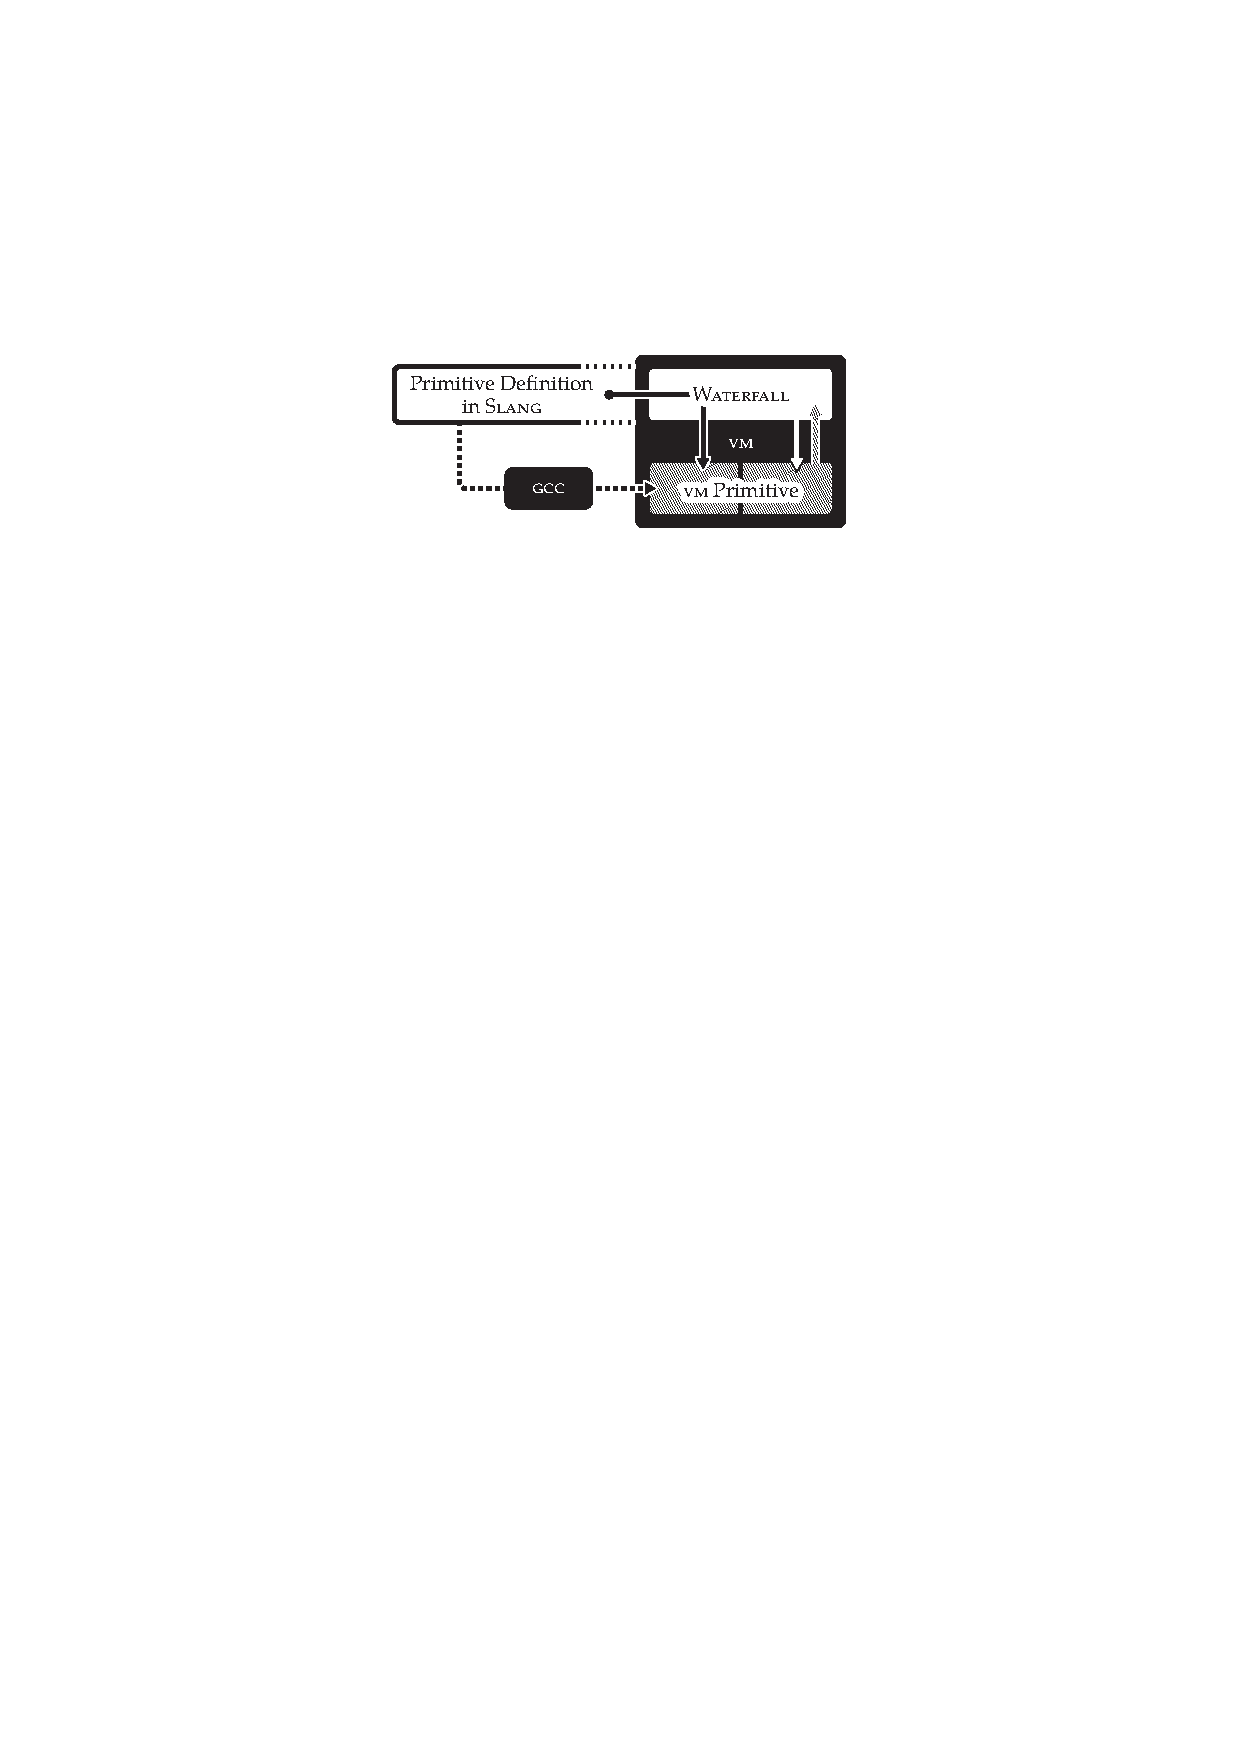
\includegraphics[scale=1.1]{waterfall-overview}
	\caption{\WF Overview}
	\figlabel{val-waterfall-overview}
\end{figure}

\noindent In this section we present \WF, a compiler toolchain that allows primitives to be changed dynamically from language-side.
We successfully use \WF to change and recompile whole \VM plugins such as the file plugin as we show in the following \secref{val-waterfall-plugins}.

% -----------------------------------------------------------------------------
\subsection{Background}
\seclabel{val-waterfall-background}
% -----------------------------------------------------------------------------

\WF is our second application on top of \B after \NB, the complete \FFI library previously presented in \chapref{ffi}.
\NB uses \B to generate the glue code between \PH and the external library.
Even though \NB is extendable it is not used to directly synthesize new functionality, the main functionality is defined the external libraries typically written in a low-level language such as C.
Interestingly, the \NB methods containing the callouts behave almost like the existing primitive methods of \PH.
These primitives define a hook into \VM-level native functionality.
In \PH the same mechanism is also used to activate plugins which are again similar to an \FFI callout from language-side.
However, primitives and plugins are statically defined and modifications happen outside \PH.
This is where the domain of \WF begins.

\WF provides infrastructure to dynamically compile and install primitives on top of the \B infrastructure at language-side in \PH.
As we will describe in more detail in the following sections, the \PH \VM is written in a metacircular fashion.
Hence the definition of plugins and primitives can be loaded in standard \PH.
Typically this happens only at compile-time of the \VM, where these definitions are exported to C and compiled to the \VM binary.
Once compiled, the original high-level description of primitives and plugins is no longer accessible from \PH.
As a consequence, existing primitives or plugins can not be changed at runtime.

\WF brings the static primitive definitions to live again.
Just loading the original definitions in \PH does not bring them back to live, even though we can now inspect the definition and browse the sources.
\WF compiles these definitions to native code and installs them with \B as new primitives.
With this infrastructure primitive and plugin modifications are not limited to \VM compilation time.

\paragraph{A Metacircular \VM Written in \Slang}

\WF is implemented in \PH which uses the \urlfootnote{\Cog \VM}{http://www.mirandabanda.org/cogblog/}, originating from the \Squeak \VM\cite{Inga97a}.
The \VM itself is written in a dialect of \ST called \Slang that is essentially limited to the functionality that can be expressed with standard C code.
\Slang serves for two purposes: a high-level C preprocessor, a interactive simulator of the \VM.
The first point has severe consequences.
\Slang basically has the same syntax as \ST but is semantically constrained to expressions that can be resolved statically at compilation or code generation time and are compatible with C.
Hence \Slang's semantics are closer to C than to \ST.
This fact is also visible in the simulator for the \VM.
If \Slang were \ST, separate parts of the \VM could be directly evaluated.
However, since \Slang is bound to C expressions, the simulator sets up a byte array as memory.
The simulated \VM then accesses this byte array as if it were the native memory.

In conclusion we see that the \PH \VM has an abstract representation of the \VM available for simulation.
This abstract representation is then used to generate C sources, already lowering the abstraction level.
After compiling the C sources the original representation of the \VM is not directly accessible anymore.
For instance, even debug symbols are usually stripped from the final binary for performance reasons.
Of course this implies that the \VM can not be changed nor directly inspected from language-side.


\paragraph{Primitives in \PH}
\PH is a highly reflective environment where classes and methods can be changed at runtime, even the current execution context is accessible.
For instance this is used to implement an exception mechanism purely at language-side in \PH.
However, some features can not be implemented at language-side.
\PH uses primitive methods, that instead of evaluating \PH-code switch to a \VM routine.
As already partially explained in \secref{benzo-vm-interaction}, whenever a method is compiled with the \ttt{primitive} pragma as shown a flag is set on the \ttt{CompiledMethod}. 
If the \VM tries to activate such a method, instead of interpreting the bytecodes it calls the corresponding function at \VM-level~\cite{Gold83a}.
We distinguish three categories of primitives based on their functionality: certain parts of the language semantics, \OS-level functionality that can not be implemented in \PH itself and a third less important category where performance is critical.

As we mentioned in the previous paragraph, these primitives are bound to the \VM and can not be changed at runtime.
However, for a certain subset of these primitives we can write language-side substitutes in pure \PH-code.
These primitives are called non-essential and are mainly used for optimization purposes. 
In contrast there are essential primitives which are for instance used during start up of the \PH environment.
Two prominent examples of essential primitives are the ones used for creating new objects or activating a block.

\paragraph{Instrumenting Primitives}
In the context of \WF we are interested in which parts of the system we can modify and thus we draw our attention to these essential primitives.
The only way to modify these primitives is by creating wrappers but that brings a new problem.
Imagine that we wrap around the primitive which creates a new object.
What happens now if the additional wrapper code needs a new object?
It will call the very same primitive that we just wrapped, without protection this causes infinite recursion.
Since technically the wrapper code should live at a different abstraction level than the original primitive we have find our selves mixing meta-levels.

The most radical approach to avoid this meta-recursion is to change the primitive externally.
In the case of \PH this means changing the \Slang sources, exporting and compiling the primitive and restarting the \PH environment on top of this changed \VM.
However, this approach stands in contrast to the reflective nature of \PH where most functionality can be changed at runtime.
Also it is not always suitable to restart the \PH process to modify a small part of the system.

%----------------------------------------------------------------------------
\subsection{\WF's Contribution}
Following the implementation overview of the \PH \VM and the differentiation of different primitives we identify two main benefits of changing \VM primitives at runtime with \WF:

\begin{enumerate}
	\item Reducing \VM complexity by implementing non-essential primitives reflectively at language-side.
	\item Dynamic instrumentation of primitives.
\end{enumerate}

\paragraph{Reducing \VM Complexity}
Low-level \VM extensions are only justified in the presence of strong performance requirements (see \secref{benzo-related}).
All non-essential primitives fall into this category since these primitives can be implemented in \PH without restrictions.
However, in certain cases for performance a language-side implementation is unsuitable.
Additionally we already know that these primitives are available as \Slang code at \VM generation time.
Using \WF, these primitives can be implemented at language-side based on the unmodified \Slang sources.
This means that these primitives become first-class citizens of the high-level environment and thus evolve with less effort.
Thus, \WF opens new possibilities of changing \PH that were previously possible only with significant overhead.

\paragraph{Essential Primitives}
For essential primitives the previous argument does not hold since a static version is needed for a correct startup of the system.
These primitives can not be directly replaced by a language-side implementation using \WF.
Even though \WF itself avoids meta-recursion by generating low-level code with \B.
However, \B itself relies on essential primitives as it is written in \PH.
This imposes certain restrictions how and when these essential primitives can be modified with \WF during system startup.
These restrictions are more related to the underlying \B infrastructure than \WF.
For instance already exposed similar limitations with the \B-based \FFI when used during startup (see \secref{ffi-startup-recursion}).
Nevertheless, nothing prevents from replacing essential primitives at runtime with customized versions, once the system startup is completed. 

\paragraph{Extended Primitive Instrumentation}
Instrumentation of essential primitives from lan\-guage-side is an error-prone task falling in many cases in non-termination due to previously described meta-recursion. 
An example of this behavior, can be observed when changing the essential \ttt{basicNew} primitive, which is responsible for instantiating new objects.
Only very limited instrumentation is possible at language-side, for instance counting how many instances have been created.
This only works since the \VM internally does not represent small integers as full objects.
However, this is only true up to some extent.
Small integers bigger than $2^{30}$ are transformed to a more expensive object representation since they no longer fit in a machine word of the 32-bit \VM. 
These big integers will use the \ttt{basicNew} primitive again as they are not implement in the \VM but in at language-side.
Thus, we are back the original problem of running into meta-recursion.
So even this very simple example has unwanted side-effects that are not directly visible.
More complex instructions tasks will inevitably suffer from the same problems.

Using reflective techniques it is possible to escape from this meta-recursion, however, with a considerable overhead.
\WF avoids these issues since the instrumentation code for primitives will be implemented at the lowest level on top of \B.
In \secref{val-waterfall-performance} we show how \WF, the \B based approach for generating primitives on the fly, outperforms the reflective solutions for primitives instrumentation. 


% -----------------------------------------------------------------------------
\subsection{Implementation}
\seclabel{val-waterfall-implementation}
% -----------------------------------------------------------------------------
\WF uses \B's mechanism for replacing primitive methods with customized versions that are nativized dynamically as described in \chapref{benzo}.
The loophole described there is exploited by \WF to enable dynamic modification of \VM behavior and hence bring primitives to life at language-side.
From a high-level point of view \WF provides two services which work transparently: 

\begin{enumerate}
	\item Compilation of \Slang code on demand (lazily).
	\item A clear interface for executing, at runtime and from language-side, the native code generated.
\end{enumerate}

\noindent The first item allows to change the code of primitives at language-side and generate the corresponding native code when needed. 
It also provides the possibility to write methods or functionality with the same \ST syntax but with a static semantic. 
It consists essentially of a transformation toolchain that transforms the \Slang sources to naitve code using a \B-based compilation toolchain.

The second item enables the execution of the dynamically generated native code.
This includes for instance the finding of addresses of \VM internal symbols and all the effort to link the two worlds, \ST and native.
\WF relies on \B for most of this low-level functionality.
In particular \NB, the \B-based \FFI presented in \chapref{ffi}, is used for interfacing with C libraries (\ttt{dlsym}). 

% -----------------------------------------------------------------------------
\paragraph{Architecture Overview}
The \WF infrastructure is mainly divided in the following two parts: the installed \Slang sources and a \B-based compilation toolchain.
The \WF compiler transforms the \Slang sources to native code through various transformation steps as show in \figref{waterfall-architecture}.
In order to work properly \WF needs the complete \Slang sources for compilation unit (primitive or plugin) to be loaded upfront.
Once loaded in the \PH image the \AST of the \Slang sources are available which form the input for the \WF compiler.
This means that it is possible to write custom plugins in \PH and transform them using \WF as long as the written \PH code uses the restricted \Slang subset.
As mentioned earlier, the major difference to normal \PH code is the lack of real polymorphism since \Slang is more like C with a \ST syntax.

Technically the \WF compiler takes over the part of the \Slang to C converter and of \GCC in the normal \VM compilation process.
\WF, much like the \Slang to C converter, has to take care of certain type information present in the \Slang sources.
For instance we extract from the type information if arguments are used by value or reference.
With this information we generate native code using a simple stack based strategy for temporary variables.
As for the part of \GCC, \WF in its current state is of course far less complex and the resulting the native code is inferior to \GCC's optimized output.
To simplify the prototype \WF only uses a simple stack strategy instead of register allocation for temporaries.
Additionally \WF does not use intermediate representations (\IR) such as static single assignment (\SSA) to perform elaborate optimizations \cite[Ch.\ 1]{Appe98a}.


% -----------------------------------------------------------------------------
\paragraph{Compilation Steps}
As shown in \figref{waterfall-architecture} the \WF compiler transforms the \AST of the \Slang input to \PH primitives.

\begin{figure}[h]
	\centering
	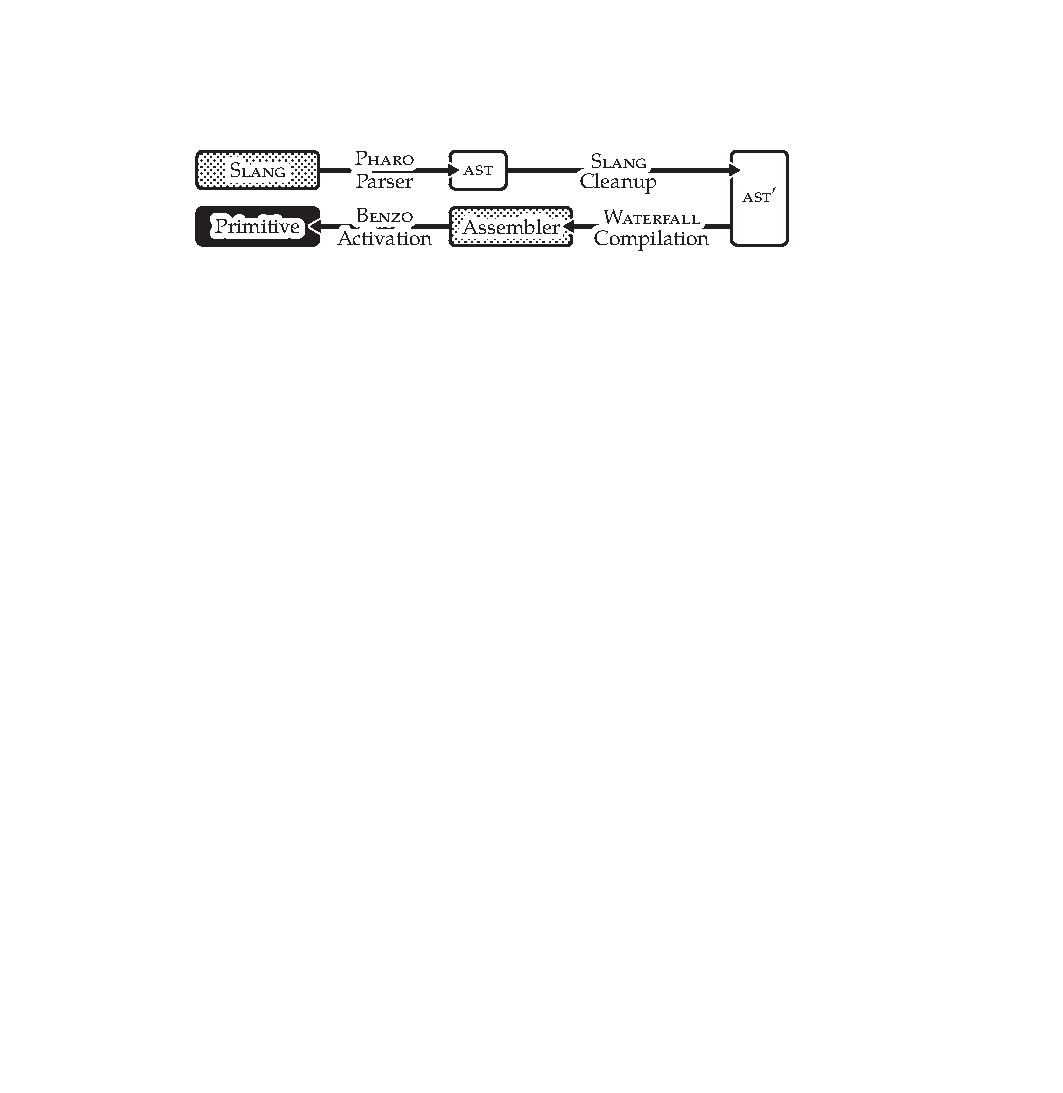
\includegraphics[scale=1.1]{waterfall-architecture}
	\caption{\WF Compilation Steps}
	\figlabel{waterfall-architecture}
\end{figure}

\noindent We divide the \WF compiler into four distinct steps:
\begin{description}
\item[\Slang to \AST:] The first step is to access the \AST of the \Slang source method which happens automatically by loading the \Slang code in the \PH image.
At this stage \WF also recursively collects the set of reachable \Slang methods.


\item[\AST Purification:] In a second step certain expressions of the original \Slang \AST are transformed into custom \WF expressions that can be easier transformed later on.
For instance \WF converts C macros that are supported in \Slang which of course only make sense when using a standard C compiler.

\item[\AST to \ASM:] The real native compilation happens in the third step where an \AST-visitor creates assembler instructions using \B's \AsmJIT.
At this point external symbols are statically resolved and directly inlined in the final \ASM code.

\item[\ASM to Primitive] Although not strictly part of the compilation, in the fourth step the final native instructions are installed as a primitive methods using \B (see \secref{benzo-benzo} for more details).
\end{description}


% -----------------------------------------------------------------------------
\paragraph{Dynamically Replacing Primitives}
After explaining the general architecture and the different compilation steps of \WF we shed some light on how the primitives are actually installed.
In reality we rely 100\% on \B for this feature.
Once the native code is generated we transform the target method to a special \B-enabled method that contains the native code.
This procedure is explained in detail in \secref{benzo-benzo} where we show the implementation details of \B.

From a user point-of-view we only have to make sure that the corresponding \Slang sources are available and then hand over that source method to \WF to compile and install it.
Once the installation is complete, the resulting \B-enabled method will contain behave like a \Slang primitive compiled with the original approach using \GCC.

% -----------------------------------------------------------------------------
\paragraph{Dynamically Replacing Plugins}
In \PH there is no real distinction between primitives and plugins as we illustrate with the following code snippets:
%
\begin{stcode}[caption={\ttt{Object>>\#basicNew} Primitive}]{3}
basicNew
  <primitive: 70>
  OutOfMemory signal.
\end{stcode}
%
\begin{stcode}[caption={\ttt{FilePlugin>>\#open:writeable:} Plugin Primitive}]{5}
open: fileName writable: writableFlag
  "Open a file of the given name, and return
   the file ID obtained."
  <primitive: 'primitiveFileOpen' module: 'FilePlugin'>
  ^ nil
\end{stcode}
%

% -----------------------------------------------------------------------------
\subsection{Validation}
\seclabel{val-waterfall-performance}
% -----------------------------------------------------------------------------
\todo{small validation introduction}


% -----------------------------------------------------------------------------
\subsubsection*{Validation of Dynamic Primitives}

For comparing performance we implement a very simple integer operation primitive (\ttt{$>$}) using three different approaches.
The first approach is the implementation with \WF.
The second is to run the language-side implementation that is triggered whenever the standard primitive failed.
Finally the fast standard primitive provided by the \VM.
We run the three approaches by measuring the cumulative time over one million primitive activations averaged over 100 runs.
The absolute numbers are less important than the relative factor between them.
We present the results of this experiment in ~\tabref{val-waterfall-performance}.
%
\begin{table}[!ht]
    \centering
    \begin{tabular}{rSS}
					& {Running Time [ms]} & {Relative Time} \\\midrule
		\VM			&   6.4(14)           & 1.0\\
		\WF	        &  22.8(17)           & \approx3.6\\
        Reflective	& 195.0(16)           & \approx30.0
    \end{tabular}
    \caption[\WF Speed Comparison: Large Integer]{Comparing running time of different implementations of integer arithmetic primitive.}
    \tablabel{val-waterfall-performance}
\end{table}
%
As expected \WF's solution outperforms pure reflective one by factor $9$ to $10$.
\WF clearly outperforms a purely reflective solution since all the meta programming overhead for the intercession mechanism is avoided. This results thus makes a whole new set of runtime extensions feasible that were previously limited by their strong performance penalty.
Furthermore the performance penalty over a completely optimized \VM solution that has extreme optimization techniques, such as inlining and register allocation, is less than a factor of $4$.
Applying standard optimization techniques, not yet implemented in \WF, will almost sure improve these numbers even more.
A more detailed analysis of \WF is available separately \cite{Char13a}.
%
\begin{table*}[h]
    \centering
    \begin{tabular}{rSS}
					                      & {Running Time [ms]} & {Relative Time} \\\midrule
        Unmodified                        &  0.28(16)           &          1 \\
        Unsafe reflective instrumentation & 21.80(33)           & \approx 78 \\
        Secure reflective instrumentation & 27.72(40)           & \approx 99 \\
        \WF-based instrumentation         &  7.72(27)           & \approx 28 \\
        \WF-based unmodified              &  7.08(23)           & \approx 25 \\
    \end{tabular}
    \caption[\WF Speed Comparison: \ttt{basicNew}]{Slowdown comparison for instrumentation of the  essential primitive \ttt{basicNew}.}
    \tablabel{val-waterfall-basicnew}
\end{table*}

\todo{add explanation of the results of \tabref{val-waterfall-basicnew}}

% -----------------------------------------------------------------------------
\subsubsection*{Validation of Dynamic Plugins}
\seclabel{val-waterfall-plugins}

\todo{Write about the File Plugin Validation}\\
\todo{Possdible Validate other plugin}


% -----------------------------------------------------------------------------
\subsection{Problems}
% -----------------------------------------------------------------------------

Currently \WF reimplements all \Slang arithmetic essential operations statically as native code templates.
The existing \JIT of the \PH \VM does exactly the same for performance reasons.
This is code duplication and should be avoided.
With the language-side \JIT compiler described on next section we can reuse the same code. Another plan for \WF is to use it for disconnecting most plugins defined at \Slang side from the \VM compilation process and dynamically compile them on a lazy approach.
Finally, adding stages to the compiler with different levels of intermediate representations and applying optimizations to each would bring its performance closer to completely low-level optimized primitives.


% -----------------------------------------------------------------------------
\subsection{Outlook}
% -----------------------------------------------------------------------------
\todo{link to the future native compilation infrastrcuture common for FFI  Benzo}\\
\todo{more performance improvements} \\
\todo{real worl applocation?} \\
\todo{better JIT interaction (leading to the following \NBJ section)}

% ===========================================================================
\newpage
\section{\NBJ: Language-side \JIT Prototype}
\seclabel{val-nabujito}
% ===========================================================================

\begin{figure}[h]
	\centering
	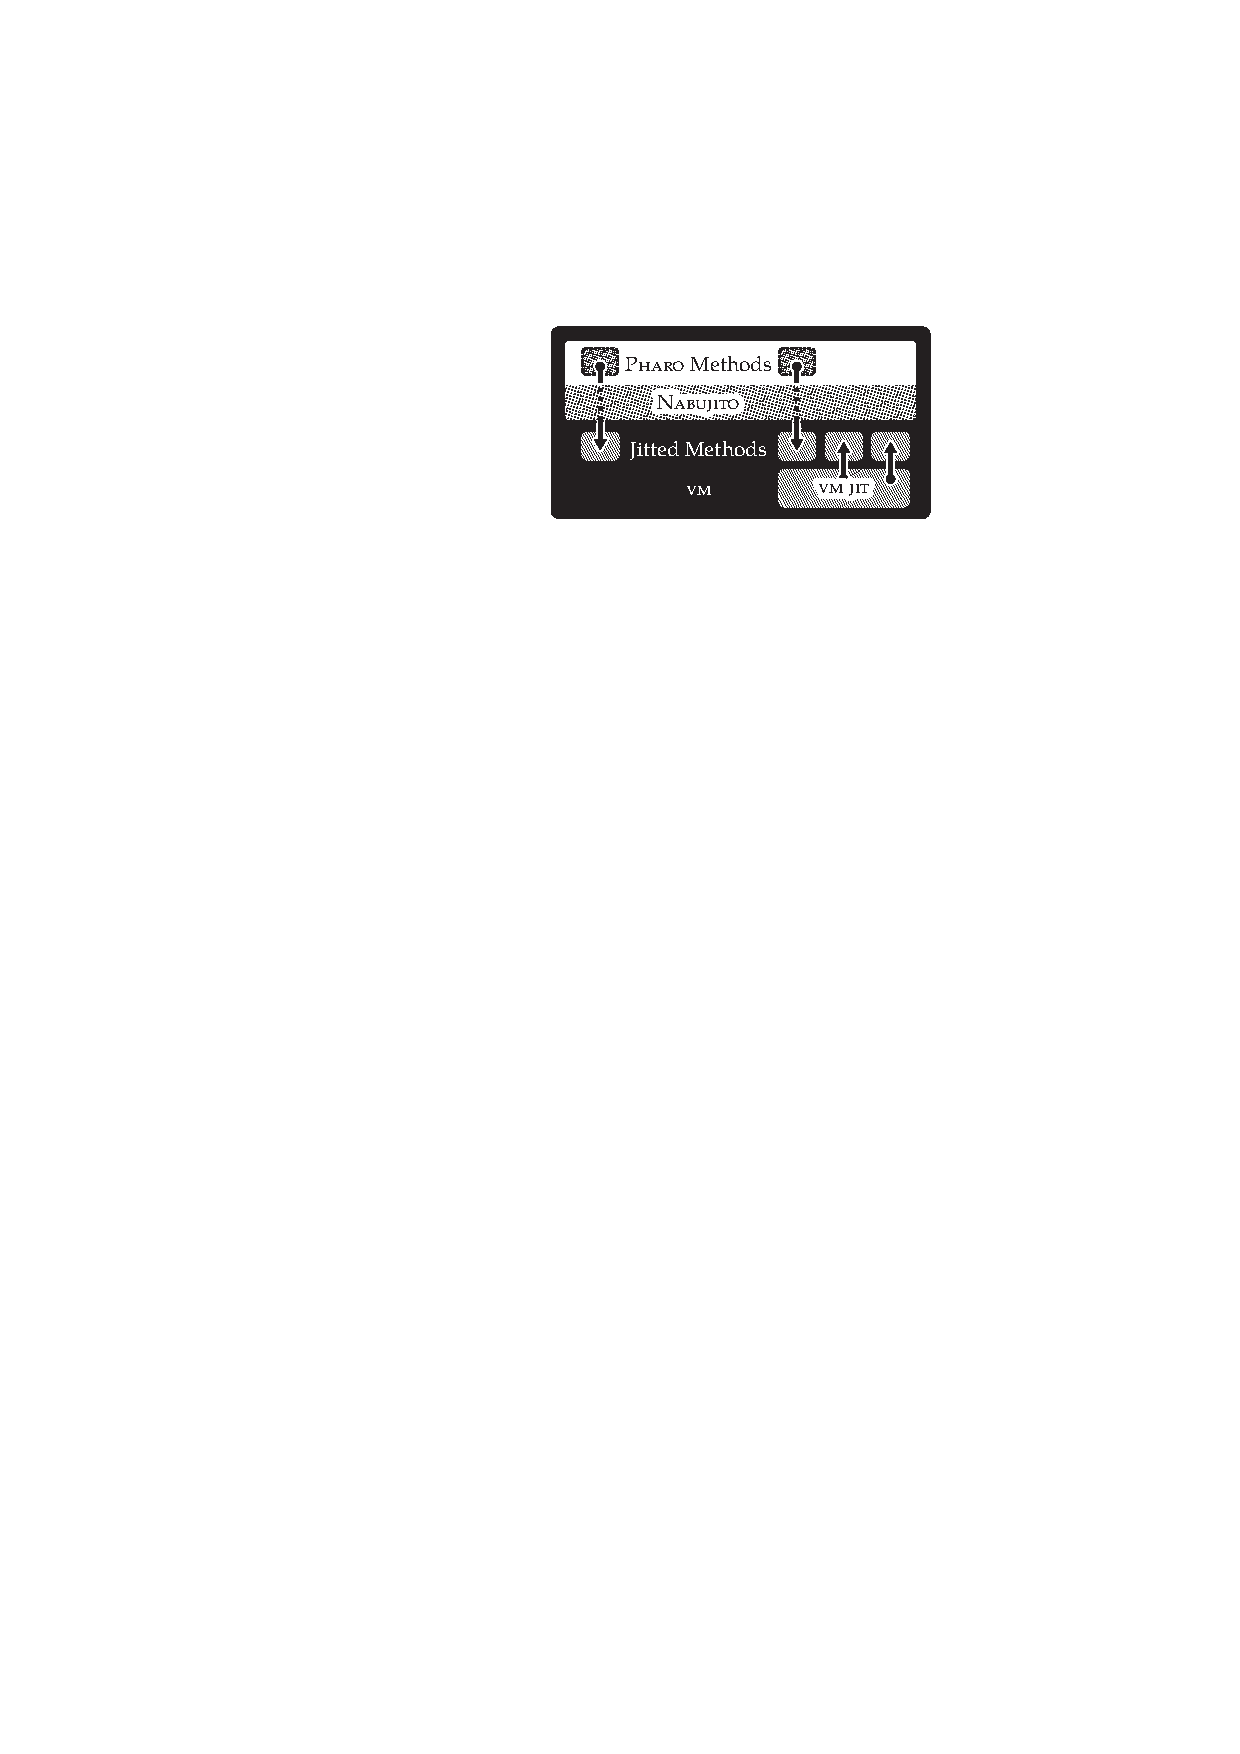
\includegraphics[scale=1.1]{nabujito-overview}
\end{figure}
\todo{Introduction}

% ---------------------------------------------------------------------------
\subsection{Background}
\seclabel{val-nabujito-background}
% ---------------------------------------------------------------------------
In this section we present \NBJ, a \B-based approach for a language-side \JIT compiler.
\NBJ goes even further than \WF using almost the same techniques.
However, instead of focusing on primitives, \NBJ generates native executable code for standard \ST methods.
Primitives tend to be more low-level, whereas \NBJ focuses on high-level \ST code. 


%----------------------------------------------------------------------------
\paragraph{The \JIT of the \PH \VM}
The \PH \VM (Cog) already comes with a \JIT that translates bytecodes to native instructions.
It transforms \ST methods into slightly optimized native code at runtime.
The main speed improvement comes from avoiding bytecode dispatching and by inlining certain known operations and primitives \cite{Ayco03a}.
The most complex logic of the \JIT infrastructure deals with the dynamic nature of the \ST environment.
Methods and classes can be changed at runtime and that has to be addressed by the \JIT infrastructure.
The \JIT compiler, by which we refer in this context to the transformation of bytecodes to native code, represents a small part of the whole infrastructure.
There exists more important stages as an additional register allocation pass to reduce the number of stack operations \cite{Mira99a,Mira11a}.
The existing \JIT infrastructure is implemented in \Slang \cite[Ch.\ 5]{Blac09a} as the rest of the \VM.

%----------------------------------------------------------------------------
\paragraph{Limitations of \VM-level \JIT Compilers}
In the context of \NBJ we separate a \JIT infrastructure into separate parts.
The major part is to have a \VM that uses stack-mapping.
In the case of a bytecode-based interpreter, we assume that the \VM provides routines to switch between a bytecode interpretation context and a low-level native execution context.
With \NBJ we move the \JIT compiler,the part that generates native code at runtime, from the \VM to the image.%, the part that generates native code at runtime, typically from bytecodes.
 Since the \JIT compiler is quite decoupled from the rest of the \JIT infrastructure we believe that a hard-coded static and low-level implementation is not optimal for several reasons:

\begin{itemize}
	\item Optimizing \ST code requires strong interactions with the dynamic environment.
	\item Accessing language-side properties from the \VM-side is hard.
	\item Changing the JIT compiler requires changes at \VM-level.
	\item The JIT reimplements primitives for optimization reasons resulting in code duplication.
\end{itemize}

\paragraph{Optimization Limitations for \PH}
In \ST methods tend to be very small and it is considered good practice to delegate behavior to other objects.
This implies that several common optimization techniques for static languages do not work well.
Dynamic method activation does not provide enough context for a static compiler to optimize methods.
Hence after inline caches and register allocation the next optimization technique is inlining.
However, inlining in a dynamic context is difficult and requires hooks at \VM-level to invalidate native code when the language-side changes.
Since in \PH, compiling a method to bytecode is handled completely with language-side code most of the infrastructure to get notified about method changes is already present.

\paragraph{Primitives in the Existing JIT}
The existing JIT reimplements the most used primitives at \VM-level.
This guarantees that the \VM stays as long as possible in the \JIT context (see \secref{benzo-jit-interaction} on page~\pageref{sec:benzo-jit-interaction}).
Additionally this enables new performance optimizations that for instance are hard to achieve with standard compliant C code.
A typical example is the integer addition which has to deal with overflow checks and conversion of tagged integers.
In \secref{val-waterfall} we describe how \WF suffers a similar constraint.
\WF manually defines such primitives in terms of native assembler instructions through the language-side \B interface.
\NBJ reuses the same optimized primitives so we rely on a single optimized definition which is shared among all native code libraries.

%----------------------------------------------------------------------------
\subsection{Implementation}
\seclabel{val-nabujito-implementation}
%----------------------------------------------------------------------------
\todo{EXTEND: Show more internals}
\todo{Add overview picture}
\NBJ is an experimental JIT implementation which replaces the bytecode to native code translation of the existing JIT infrastructure with a dynamic language-side implementation.
\NBJ is implemented mainly with a visitor strategy over the existing intermediate bytecode representation. 
Additionally we reimplemented vital native routines for the JIT which are not directly exported by the \VM using \B. 
Nabujito relies on the following \VM-level infrastructure to manage and run native code for any \PH method:

\begin{itemize}[noitemsep]
	\item Fixed native code memory segments.
	\item Routines for switching contexts.
	\item Native stack management.
\end{itemize}


\paragraph{\NBJ Compiler Steps}
\todo{Overview Figure of the input / transformation steps} \\
\todo{Almost Reified Cog Routines} \\
\todo{CogMethod patching problem leading to the following parargraph}


\paragraph{Dynamic Code Generation}
To simplify the implementation we decide to manually trigger JIT compilation.
For primitives known by \WF we rely on that infrastructure to generate the native code.
For standard methods \NBJ takes the bytecodes and transforms them to native code.
It also applies optimizations such as creating low-level branches for \ST level branching operations like \ttt{ifTrue:}.
Optimizations for additional methods are all implemented flexibly at language-side.
Wherever possible, we reimplement the same behavior as the existing native \JIT compiler.
Eventually the native code is ready and \B attaches it to the existing compiled method.
When the language-side jitted code is activated \B ensures that we do not have to leave the \JIT execution mode, and thus we can call methods at the same speed as the existing \JIT.
\todo{figure showing an extended method installation into \JIT space}


\paragraph{The \Cog \JIT}
To understand the implementation issues of \NBJ we have to dive into the details of \PH's \JIT.
\PH uses a flavor of the \Cog \VM which evolved in several steps from a simple bytecode interpreter.
A successful and fast \JIT implies a \VM that uses the native stack.

The original \ST-80 blue book implementation foresees a spa\-ghet\-ti-stack where all contexts are normal objects on the heap.
This design simplifies the \VM implementation significantly since there is no special treatment necessary for blocks.
Also this makes it rather easy to implement \PH's feature to access the current context using the special \ttt{thisContext} variable.
However, the obvious down side of this implementation is the massive stress on the \GC.
For each message send a new context has to be allocated and on each return contexts have to be reclaimed.
It would naturally be more efficient to use the native stack which allows for cheap allocation and precise reclaiming of method context.
While this mapping can be done rather easily there are three properties of \PH that make this hard: blocks, non-local returns and the mentioned \ttt{thisContext}.
Eliot Miranda eventually succeeded to implement an efficient mapping scheme for the \Cog \VM that is based on the original work done by Peter Deutsch and Allan Schiffman \cite{Deut84a}.

Even so the basic concepts of the native stack mapping are easy to understand the final implementation is rather tricky.
Real closures that outlive their outer method activation context make the mapping tricky.
At the same time all the reflective capabilities to modified the stack from within \PH have to be supported.
\cb{shall we explain more here?}.


\todo{Step 2: transform bytecodes to native code}\\
\todo{Step 3: Trampolines to jump back and forth between native activated scheme and bytecode interpreter based approach}\\
\todo{Step 4: Minor summary of the how the ICs work in the \JIT}

\begin{figure}[h]
	\centering
	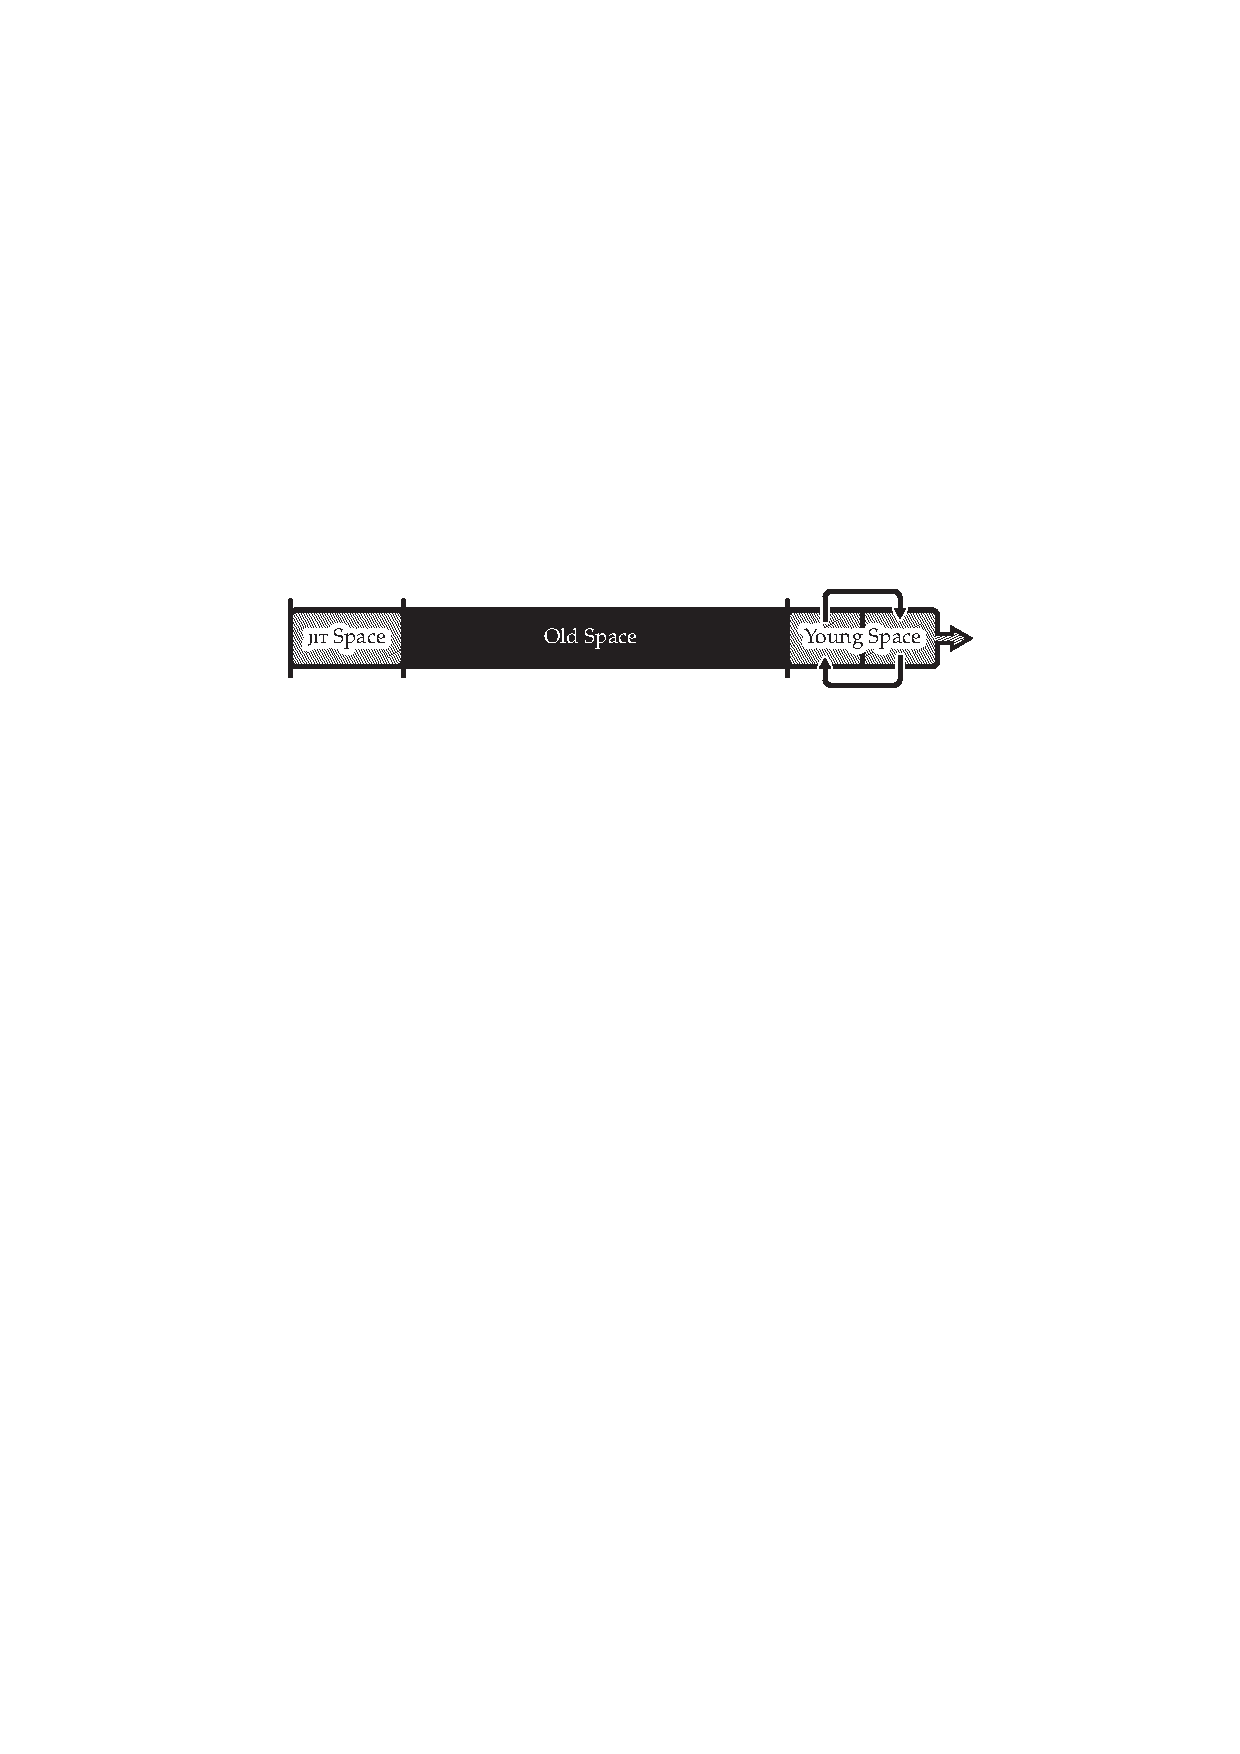
\includegraphics[scale=1.1]{cog-memory}
	\caption[\Cog Memory Model Overview]{\Cog Memory Model Overview: Fixed-sized \JIT space, slow changing old space and fast young space.}
	\figlabel{cog-memory}
\end{figure}

\begin{figure}[h]
	\centering
	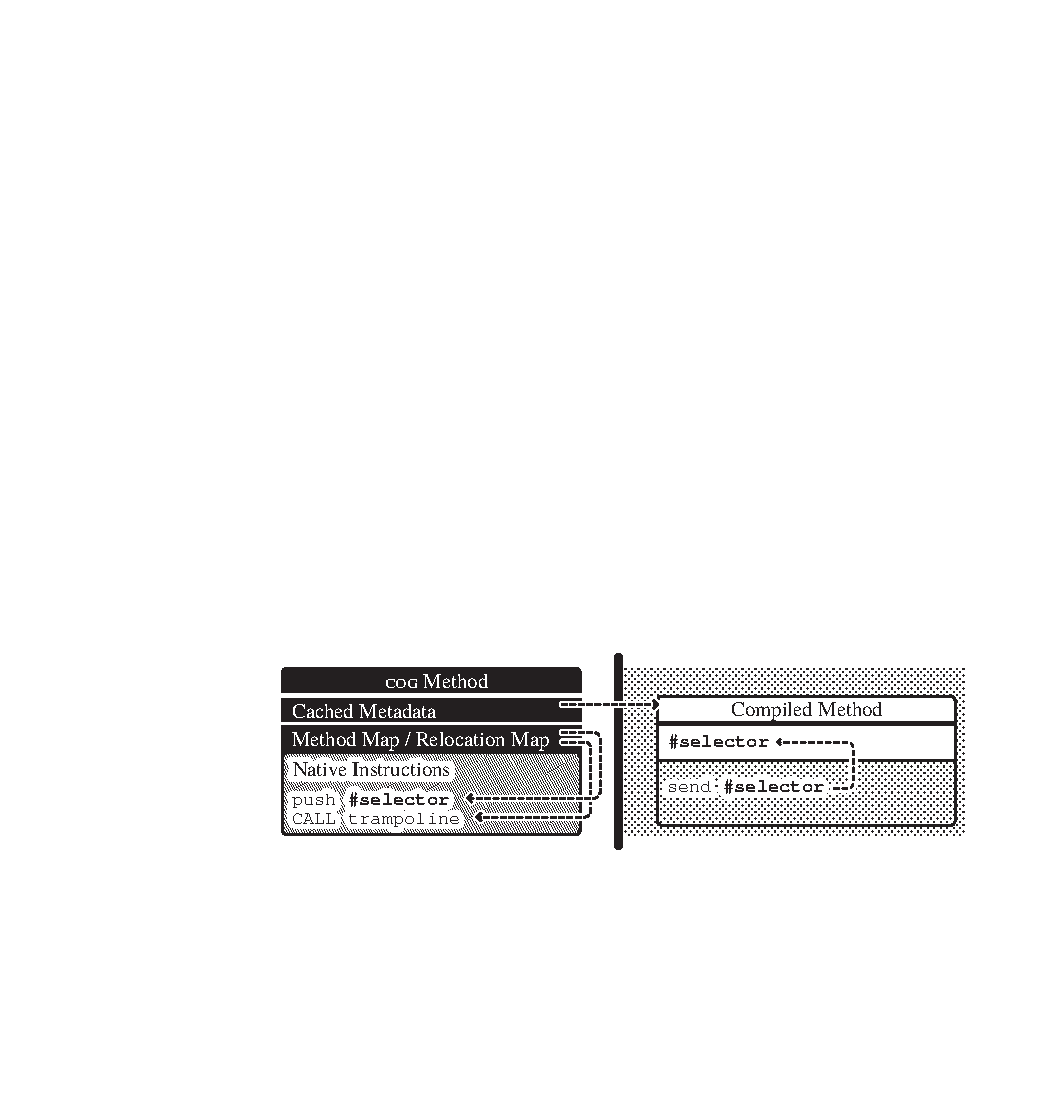
\includegraphics[scale=1.1]{cog-method}
	\caption[\Cog Method]{\Cog Method: Compiled method representation at \JIT-level residing in the \JIT memory space.}
	\figlabel{cog-method}
\end{figure}

\paragraph{Overcoming the Missing \VM Interface for the \JIT}
\todo{why do we need patch methods?}\\
\todo{Explain how the patch methods work}\\
\todo{give example of the assember of a simple method with the patch call}

% -----------------------------------------------------------------------------
\subsection{Validation}
\seclabel{val-nabujito-performance}
% -----------------------------------------------------------------------------

\todo{missing intro}

% -----------------------------------------------------------------------------
\subsubsection*{Compilation Time}


The performance evaluation for our \B-based \JIT compiler is focused on the language-side code-generation part.
\NBJ essentially generates the same native code as the \VM-level \JIT, hence there is no performance difference at evaluation time.
However, \NBJ is clearly slower during the warm-up phase.
Compilation of the native instructions will take considerably more time compared to the \VM-level implementation of the same bytecode to assembler transformation.
The cost of transforming the bytecodes to native code at \VM-level can be measured in native instructions, whereas the unit at language-side is bytecodes.
However, we point out again, that this is a one-time overhead.
From the in-production experience of \NB, the \B-based \FFI (see \secref{ffi-evaluation}), we know that these costs amortized, especially for long-term applications.
Instead of focusing on the final performance of the generated code, we present the compilation time compared to the normal \PH bytecode compiler, which also resides at language-side.

\begin{table}[!ht]
    \centering
    \begin{tabular}{rS}
                      & {Compilation Time [ms]} \\\midrule
        \PH Compiler  & 71(1) \\
        \NBJ          & 73(1)
    \end{tabular}
    \caption[\NBJ Compilation Speed]{Compilation efforts of the standard \ST compiler in \PH and \NBJ for the a simple method returning the constant \ttt{nil}.}
    \tablabel{val-nabujito-performance-small}
\end{table}

\noindent In \tabref{val-nabujito-performance-small} we compare the compilation speed of the standard \PH compiler and \NBJ.
We measure the accumulated time spent to compile the method 1000 times.
The average and deviation are taken over 100 runs. 
The \PH compiler takes source code as input and outputs \ST bytecodes.
\NBJ takes bytecodes as input and outputs native code.

We see that in the simple case displayed in \tabref{val-nabujito-performance-small} \NBJ's compilation speed lies within the same range as the standard \ST compiler.
We expect that in the future we apply more low-level optimizations and thus increase the compilation time of \NBJ.
However, we have shown in the performance evaluation for \NB, the \B-based \FFI, in \secref{ffi-evaluation} that even a rather high one-time overhead is quickly amortized.
Furthermore with \ST's image approach the generated native code is persistent over several sessions.
A subsequent restart of the same runtime will not cause the \JIT to nativize the same methods it did during the last launch.
Hence our approach is even valid for short-timed script-like applications as most of the methods will already be available in optimized native code from a previous run.

% -----------------------------------------------------------------------------
\subsubsection*{Per Method Comparison}
\todo{choose simple enough methods that we can compile with nabujito: currently only + works}


% -----------------------------------------------------------------------------
\subsection{Problems}
\seclabel{val-nabujito-problems}
% -----------------------------------------------------------------------------
\paragraph{Hidden \VM Internals}
\todo{backref to patch methods}\\
\todo{maintenance problem: \NBJ harcodes the \VM interaction}


\paragraph{Debugging Cycle}
\todo{Missing tools to directly interact with benzo / the real vm} \\
\todo{missing small assembler tests} \\
\todo{reactivate the VM simulator infrastructure}

\paragraph{Missing Optimizations}
One major performance optimization missing in both, the original \PH \VM-level \JIT and \NBJ, is inlining. 
By inlining we are able to create methods that are potentially big enough for optimizations.
However, inlining is a difficult task in a highly dynamic language such as \ST or \Self \cite{Cham89a}. 
Efficient inlining can only be performed with sufficient knowledge of the system. 
Accessing this high-level information from within the \VM is cumbersome and requires duplication of language-side reflective features.
The \JIT lives on the same level as the information it needs relying on the already present reflective features of \ST.


% ===========================================================================
\section{Outlook}
% ===========================================================================

\todo{Common problem: missing debugging infrastructure} \\
\todo{\WF and \NBJ share the same problems} \\
\todo{For speed a proper \JIT interface is missing } \\


% ===========================================================================
\section{Summary}
% ===========================================================================


% =============================================================================
% empty version for the main document, where all the chapters are compiled together